\documentclass{kis}
%\addbibresource{references.bib}

\newacronym{pwm}{PWM}{Pulsbreitemodulation}

\title{Laborbericht}

\begin{document}
\maketitle
\pagenumbering{Roman}
\setcounter{tocdepth}{2}
\tableofcontents
\listoffigures
\clearpage
\pagenumbering{arabic}

\section{Systemanalyse}

\subsection{Sensoren}
\subsubsection{Hallsonde} 
Eine Hallsonde (benannt nach ihrem Erfinder Edwin \textsc{Hall}) ist ein Sensor zur Messung von Magnetfeldern. Auch wenn solche Messinstrumente prinzipiell auch analoge Messungen durchführen kann, wird er in dieser Anwendung ledglich als digitaler Sensor verwendet. An der Drehscheibe ist eine magnetische Markierung angebracht, wodurch eine an dem festen Aufbau angebrachte Hallsonde einen entsprechenden Logikpegel erzeugen kann. Diese Markierung ist so angebracht, dass an dem Digitalpin ein Low-Pegel anliegt, wenn sich das Loch der Drehscheibe über der Senke in dem Aufbau befindet.  Die Hallsonde wird in diesem Aufbau also verwendet, um die Position des Lochs zu bestimmen. Wenn an dem Digitalpin der Hallsonde eine 1-0-Flanke detektiert wird, beginnt das Loch in der Drehscheibe sich mit dem Loch in der Senke zu überschneiden.

\subsubsection{Photosensor}
Auf der Unterseite der Drehscheibe befindet sich ein Muster ähnlich wie bei einem Glücksrad, aus sechs weißen und sechs schwarzen, jeweils alternierend Bereichen. Ferner befindet sich unter der Drehscheibe ein Photosensor, welcher verwendet werden kann, um die Farbe über diesem zu bestimmen. Auch hier ist der Sensor, obwohl er prinzipiell auch analog messen könnte, mit einem Digitalpin verbunden, sodass damit entsprechend der Farbe -- schwarz oder weiß -- einen High- oder Low-Pegel gemessen werden kann. Damit kann durch den Photosensor die Drehgeschwindigkeit der Scheibe gemessen werden. Aufgrund der Periodizität des ausgegeben Signals (siehe Abb. \ref{fig:photosensor}) kann aus dem Photosensor jedoch der aktuelle Drehwinkel nicht eindeutig bestimmt werden.

\begin{figure}
	\centering
	\input{photosensor.pdf_tex}
	\caption[Signal des Photosensors bei einer Umdrehung der Scheibe.]{Signal des Photosensors bei einer Umdrehung der Scheibe. Der Duty Cycle der periodischen Funktion beträgt genau $\frac{1}{2}$.}
	\label{fig:photosensor}
\end{figure}

Offensichtlich kann auch die Hallsonde die Drehgeschwindigkeit der Scheibe messen, doch der Photosensor ist für diese Aufgabe besser geeignet. Während die Hallsonde zur Bestimmung der Drehgeschwindigkeit mindestens eine volle Umdrehung benötigt, kann der Photosensor diese Messung in $\frac{1}{6}$ Umdrehung (wenn ein schwarz-weiß-Zyklus bestimmt wird) oder gar in nur $\frac{1}{12}$ Umdrehung (wenn nur ein schwarzes \emph{oder} ein weißes Feld verwendet wird) durchführen. Da außerdem die Entschleunigung der Scheibe gemessen werden sollte, wofür bei Verwendung der Hallsonde noch eine weitere Umdrehung benötigt wird, würde bei Verwendung der Hallsonde also inakzeptabel viel Zeit zwischen Auslösen durch den Nutzer und Fall der ersten Kugel vergehen. Würde sich die Scheibe mit der niedrigsten spezifikationsgerechten Drehzahl von 0,2~U/s drehen, würde diese Zeitdifferenz mindestens 10~s betragen.

Kurz zusammengefasst kann die Hallsonde sowohl die gewünschte Position als auch die Drehzahl bestimmen, während der Photosensor lediglich die Drehzahl bestimmen kann, für diese eine Aufgabe aber deutlich besser geeignet ist.

\clearpage
\subsection{Aktoren}
\subsubsection{Servoantrieb}
\begin{wrapfigure}[12]{r}{0.5\textwidth}
	\raggedleft
	\vspace*{-0.5\baselineskip}
	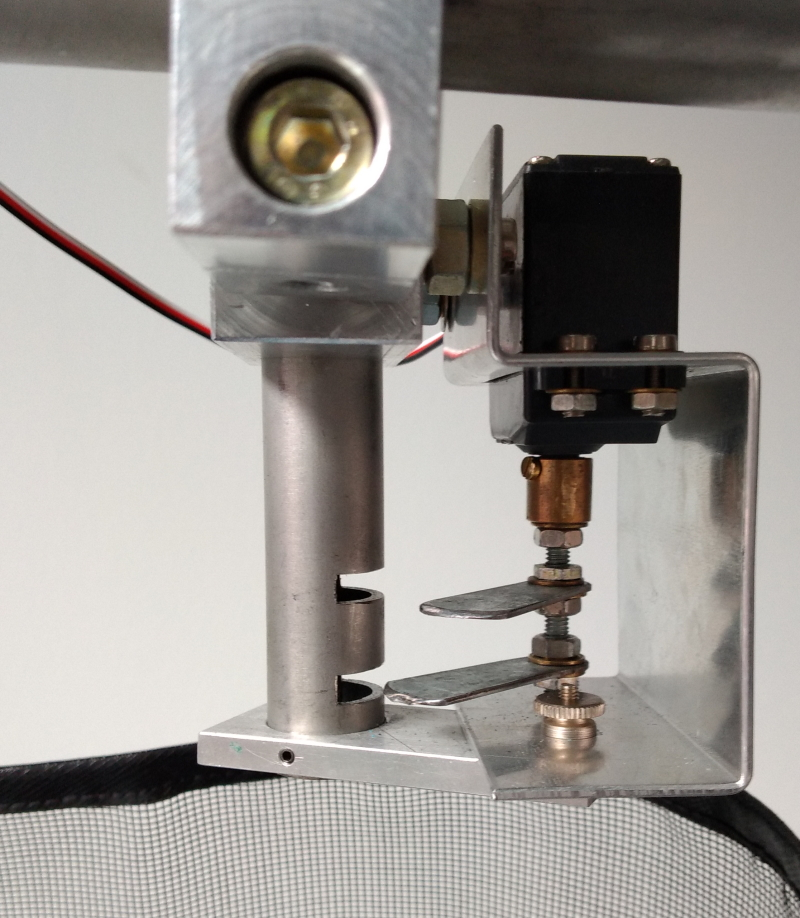
\includegraphics[width=0.9\linewidth]{IMG_20200525_171143701.jpg}
	\caption[Vorrichtung zum Abwurf der Kugeln]{Durch den Servoantrieb betriebene Vorrichtung zum Abwurf der Kugeln.}
\end{wrapfigure}
Bei einem Servoantrieb, wie er in dem Aufbau verwendet ist, erfolgt die Vorgabe der Sollgröße (d.h. des Winkels) üblicherweise über ein \gls{pwm}-Signal; durch eine interne Regelschleife wird der Servomotor auf die vorgegebene Position ausgeregelt. Da die Blackbox die Erzeugung des entsprechenden Signals nicht übernimmt, muss dies direkt durch den Arduino geschehen. Dafür existiert die \texttt{Servo}-Library, welche das \gls{pwm}-Signal für einen Winkel zwischen 0° und 180° erzeugt.
An der von dem Servoantrieb angetriebenen Welle befinden sich zwei versetzt angebrachte Zungen aus Metall, durch welche die Metallkugeln nacheinander freigesetzt werden können. Dabei sind zwei Stellungen von besonderer Wichtigkeit.

\begin{itemize}
\item[35°:] Hier blockiert die untere Zunge die unterste Kugel, die obere Zunge blockiert jedoch nichts, sodass eine oben eingeworfene Kugel in die Kammer fällt und dort verbleibt, bis die untere Zunge sie freigibt.
\item[50°:] Nun gibt die untere Zunge die Kammer frei, sodass die dort gelagerte Kugel herausfällt. Durch die Versetzung der beiden Zungen blockiert nun die obere Zunge die Kammer, sodass nur die eine in der Kammer befindliche Kugel freigesetzt wird und alle weiteren oben eingeworfenen Kugeln über der Kammer verbleiben.
\end{itemize}

Dies bedeutet, dass der Servoantrieb standardmäßig auf 35° gesetzt werden soll. Zur Freisetzung einer Kugel muss der Servoantrieb auf 50° ausgelenkt und anschließend wieder auf 35° gesetzt werden.

Eine mögliche Fehlerquelle, welche bereits bei der ersten Systemanalyse auffällt, ist die nichtvernachlässigbare Reaktionszeit der Abwurfvorrichtung aufgrund der langsamen Stellgeschwindigkeit des Servoantriebs. Dies hat eine höhere Zeitdifferenz zwischen (vermeintlichem) Abwurf und Auftreffen im Loch der Drehscheibe zur Folge, welche aber für alle Drehzahlen als konstant angenommen werden kann. Außerdem folgt daraus, dass die Zeit zum Auftreffen der Kugel experimentell bestimmt werden muss. Zwar kann die Fallzeit selbst aus den Gesetzen der Physik hergeleitet werden:
$$s = \frac a2t^2+vt+s_0~\text{mit}~v=0;~ s_0=0;~ s=0,72~\text{m};~ a=g=9,81~\frac{\text{m}}{\text{s}^2}$$
\begin{align*}t_\text{Fall} &= \sqrt{\frac{2s}{a}}\\
&= \sqrt{\frac{2\cdot0,72~\text{m}}{9,81~\frac{\text{m}}{\text{s}^2}}}\\
&= 0,38~\text{s}\end{align*}
Diese Zeit würde jedoch nicht die nichtvernachlässigbare Stellzeit des Servoantriebs einschließen. Diese muss experimentell bestimmt werden. Dabei ergab sich:
\begin{align*}t &= t_\text{Stell} + t_\text{Fall}\\
&= 0,46~\text{s}\end{align*}

\subsection{Kommunikation mit dem Nutzer}

\subsubsection{Serielle Schnittstelle}
Das Arduino-Board kommuniziert über eine serielle USB-UART-Schnittstelle mit dem PC. Dadurch können durch eine entsprechend konfigurierte Software auf dem PC Daten vom Arduino empfangen und zum Arduino gesendet werden.

\subsubsection{Trigger}
Mit der Blackbox ist über ein Kabel ein kleines Bediengerät verbunden, welches einen Knopf besitzt. Wenn der Knopf darauf gedrückt wird, liegt an dem entsprechenden Pin ein High-Pegel an; ansonsten ein Low-Pegel. Dieses Bediengerät kann sehr gut zum Start der Durchführung verwendet werden. 

\subsubsection{Sonstiges}
\paragraph{Buttons}
Zwei Buttons auf dem Arduino-Board. Durch diese wird erwartungsgemäß ein High-Pegel an dem entsprechenden Pin angelegt, wenn sie gedrückt werden, und ansonsten ein Low-Pegel.
\paragraph{Kippschalter}
Der auf der Blackbox angebrachte Kippschalter legt in der unteren Stellung (\glqq Controller\grqq) einen High-Pegel an dem Pin an; in der oberen Stellung (\glqq Direct\grqq) sowie in der Zwischenstellung einen Low-Pegel.
\paragraph{LEDs}
LED 1 leuchtet gelb, LED 2 leuchtet grün. Bei einem angelegten High-Pegel leuchten die LED jeweils, bei einem Low-Pegel bleiben sie aus. Der Pin der LED 2 ist außerdem mit der onboard-LED des Arduino-Boards verbunden.

\subsection{Machbarkeitsanalyse}
Ein Test mit Auslösung der Kugeln direkt über den Trigger zeigte, das selbst \emph{bei Stillstand der Scheibe} nicht alle Kugeln zuverlässig das Loch trafen. Selbst bei Stillstand der Scheibe verfehlten zwischen $\frac13$ und $\frac12$ der abgeworfenen Kugeln die Senke und prallten an dem äußeren Rand des Lochs in der Scheibe ab.

Dieses Verhalten ist einzig und allein dem physikalischen Aufbau des Systems\footnote{Es wurde der Aufbau im Raum Z 2045 gewählt.} geschuldet. Die Software wird nicht in der Lage sein, dies zu korrigieren, wodurch bereits bei ersten, einfachen Tests des Aufbaus berechtigte Zweifel an der Machbarkeit aufkommen.

Der Versuchsaufbau besitzt folgende Probleme, welche Grund für dieses Verhalten sein können.
\begin{itemize}
	\item Der Aufbau steht nicht perfekt gerade, sondern ist um einen geringen Winkel geneigt, wodurch die Kugel weiter außen auftrifft als erwartet.
	\item Die Lagerung der Scheibe besitzt relativ viel Spiel, sodass sich die Scheibe unrund dreht.
	\item Das Loch in der Scheibe ist nicht perfekt konzentrisch.
	\item Das Rohr in der Abwurfvorrichtung, durch welche die Kugeln fallen, besitzt ein Übermaß, sodass nicht gewährleistet werden kann, dass die Kugel mittig durch die Vorrichtung fällt.
\end{itemize}

\section{Design}
\subsection{Wahl der Randbedingungen}
\paragraph{Drehgeschwindigkeit}
Es werden folgende Schwellwerte für die Drehgeschwindigkeit festgelegt:
\begin{itemize}
	\item Langsam: $t_r>3~\text{s/U}$
	\item Mittelschnell : $1~\text{s/U}\leq t_r\leq 3~\text{s/U}$
	\item Schnell: $t_r<1~\text{s/U}$
\end{itemize}

\paragraph{Aufbau}
Es wurde der Aufbau im Raum Z 2045 gewählt. Die Scheibe wird entgegen dem Uhrzeigersinn gedreht.

\subsection{Grobentwurf}
Der Entwurf sowie die Implementierung werden Anhand des in Abb. \ref{fig:lösungsstack} gezeigten Lösungsstacks durchgeführt, wobei der Hardwarelayer bereits durch den Kugelfall-Aufbau, die Blackbox und das Arduino-Shield gegeben ist. Der hardwarenahe Softwarelayer soll einige wichtige Funktionen des Aufbaus gegenüber dem Anwendungslayer abstrahieren, während der Anwendungslayer den Algorithmus zum spezifikationsgerechten Abwurf der Kugeln darstellt.

\begin{figure}
	\centering
	\newcolumntype{Y}{>{\centering\arraybackslash}X}
	\renewcommand{\arraystretch}{1.7}
	\begin{tabularx}{0.8\textwidth}{|Y|}
		\hline
		\large Anwendungslayer\\
		\small Algorithmus zum Abwurf der Kugeln\\
		\hline
		\large Hardwarenaher Softwarelayer\\
		\small Funktionen zur Abstraktion der Hardware\\
		\hline
		\large Hardwarelayer\\
		\small Verbindung zum Testaufbau selbst\\
		\hline
	\end{tabularx}
	\caption{Lösungsstack.}
	\label{fig:lösungsstack}
\end{figure}

\subsection{Hardwareanbindung}
Konkret bestehen die Aufgaben des hardwarenahen Softwarelayers aus folgendem:

\paragraph{Bestimmung der Drehgeschwindigkeit der Scheibe}
Für diese Aufgabe wird gemäß der Vorbetrachtung der Photosensor verwendet. Durch Messung der für einen schwarz-weiß-Zyklus benötigten Zeit und Multiplikation mit dem Faktor 6 kann die Zeit für eine volle Umdrehung bestimmt werden.

\paragraph{Bestimmung der Abbremsung der Scheibe}
Um die Abbremsung der Scheibe zu bestimmen, müssen zwei schwarz-weiß-Zyklen gemessen werden und daraus die Zeitdifferenz bestimmt werden. Daraus kann, wieder nach Multiplikation um den Faktor 6 die Zeit bestimmt werden, welcher sich die Zeit für eine Umdrehung pro Umdrehung erhöht. Tatsächlich sinkt die Geschwindigkeit der Scheibe nicht linear ab -- bei einem durch Reibungs- und Luftwiderstand verzögertem Objekt sinkt die Geschwindigkeit in Form einer Exponentialkurve -- doch die Linearisierung ist hier eine akzeptable Approximation.

\paragraph{Bestimmung der Position des Lochs}
Die Position des Lochs kann durch eine Warte-Funktion realisiert werden, welche die Ausführung des Programms so lange blockiert, bis an dem Digitalpin der Hallsonde die zuvor erläuterte 1-0-Flanke beginnt. Die Entscheidung, wann die Kugel auf Grundlage dessen abgeworfen werden soll, obliegt anschließend dem Anwendungslayer. 

\subsection{Algorithmus zum Abwurf der Kugeln}

\section{Implementierung}

\subsection{Implementierung des Entwurfs}
\subsubsection{Hardwareanbindung}
In der Embedded-Programmierung gilt es immer, ein sinnvolles Gleichgewicht zwischen Abstraktion und Performanz zu finden. Bei 32~kB Flash-Speicher und nur 2~kB RAM kann sich überflüssige Objektorientierung, wenngleich sie unbestreitbar die Lesbarkeit des Codes verbessert, eher kontraproduktiv auswirken.

Um die zugrundeliegende Hardware zu abstrahieren, wird eine Header-Datei erstellt, welche einige Funktionen und Struts bereitstellt und von dem Anwendungslayer eingebunden werden kann. Dieser Ansatz entspricht auch im Wesentlichen dem Industriestandard bei Embedded-Software.

\paragraph{Vorbereitung der Hardware}
Die Pinbelegung wird ebenfalls in der Header-Datei spezifiziert. Die Funktion \texttt{setupHardware()} initialisiert die Pins und legt die Baudrate für die serielle Schnittstelle fest.

\paragraph{Messung der Drehung der Scheibe}
Es ist nicht besonders sinnvoll, zwei separate Funktionen zur Messung der Drehgeschwindigkeit und zur Messung der Abbremsung zu haben -- wenn die Abbremsung gemessen werden soll, muss dazu die Drehgeschwindigkeit ebenfalls gemessen werden. Um dies zu realisieren, existiert die \texttt{rotationMeasure()}-Funktion, welche über eine als Argument zu übergebende Anzahl schwarz-weiß-Zyklen (wenigstens zwei) die Drehgeschwindigkeit und die Abbremsung der Scheibe misst und einen Struct mit den Attributen \texttt{time} (Einheit: ms/U) und \texttt{deceleration} (Einheit: ms/U$^2$) zurückgibt.

Die Funktion ist als Pseudocode in Abbildung \ref{fig:pseudo-dreh} gezeigt.

Diese Funktion sorgt außerdem dafür, die LEDs entsprechend der gemessenen Drehgeschwindigkeit ein- und auszuschalten. Bei langsamer Drehung leuchtet die grüne LED, bei mittelschneller Drehung leuchten beide LEDs und bei schneller Drehung leuchtet nur die orangene LED.

\begin{figure}
\lstset{basicstyle=\small\ttfamily,tabsize=4}
{\singlespacing
\begin{lstlisting}[frame=single]
function measureRotation() => integer, integer

	# sicherstellen, dass Messung nicht mitten auf Feld beginnt
	while PhotoSensorPin = 1 loop
		idle
	end while
	while PhotoSensorPin = 0 loop
		idle
	end while

	# zwei 1-0-Zyklen messen
	tBeforeFirstCyc := millis()

	for i from 0 to 2 loop
		while PhotoSensorPin = 1 loop
			idle
		end while
		while PhotoSensorPin = 0 loop
			idle
		end while
		
		if i = 1 then
			tAfterFirstCyc := millis()
		end if
	end for	
	
	tAfterSecondCyc := millis()
	
	t_r1 := 6 * (tAfterFirstCyc - tBeforeFirstCyc)
	t_r2 := 6 * (tAfterSecondCyc - tAfterFirstCyc)
	
	t_r := (t_r1 + t_r2) / 2
	delta_t_r := (t_r2 - t_r1)
	
	return t_r, delta_t_r
	
end function
\end{lstlisting}
}
\caption{Pseudocode zur Bestimmung der Drehgeschwindigkeit.}
\label{fig:pseudo-dreh}
\end{figure}

\paragraph{Bestimmung der Position des Lochs}
Die Funktion \texttt{awaitHallSensorPosition()} wartet auf die nächste 1-0-Flanke des Pins der Hallsonde und blockiert die Ausführung des Programms währenddessen. 

\begin{figure}
\lstset{basicstyle=\small\ttfamily,tabsize=3}
{\singlespacing
\begin{lstlisting}[frame=single]
function awaitHallSensorPosition()

	# Anfang eines High-Pegels erwarten
	while HallSensorPin = 0 loop
		idle
	end while
	
	# Ende des High-Pegels erwarten
	while HallSensorPin = 1 loop
		idle
	end while
	
	# Prozessor freigeben sobald der High-Pegel vorbei ist
	return
	
end function
\end{lstlisting}
}
\caption{Pseudocode zur Bestimmung der Position des Lochs.}
\label{fig:pseudo-loch}
\end{figure}

\subsection{Fehlerfindung und -behebung}

\subsection{Ergebnisanalyse}

\appendix
%\addcontentsline{toc}{section}{Literatur}
%\printbibliography
\end{document}